%%%%%%%%%%%%%%%%%%%%%%%%%%%%%%%%%%%%%%%%%%%%%%%%%%%%%%%%%%%%%%%%%%
%%%%%%%% ICML 2013 EXAMPLE LATEX SUBMISSION FILE %%%%%%%%%%%%%%%%%
%%%%%%%%%%%%%%%%%%%%%%%%%%%%%%%%%%%%%%%%%%%%%%%%%%%%%%%%%%%%%%%%%%

% Use the following line _only_ if you're still using LaTeX 2.09.
%\documentstyle[icml2013,epsf,natbib]{article}
% If you rely on Latex2e packages, like most moden people use this:
\documentclass{article}

% For figures
\usepackage{multirow}

\usepackage{graphicx} % more modern
%\usepackage{epsfig} % less modern
\usepackage{subfigure} 

% For citations
\usepackage{natbib}
\usepackage{subfigure}
% For algorithms
\usepackage{algorithm}
\usepackage{algorithmic}

% As of 2011, we use the hyperref package to produce hyperlinks in the
% resulting PDF.  If this breaks your system, please commend out the
% following usepackage line and replace \usepackage{icml2013} with
% \usepackage[nohyperref]{icml2013} above.
\usepackage{hyperref}
\nocite{*}

% Packages hyperref and algorithmic misbehave sometimes.  We can fix
% this with the following command.
\newcommand{\theHalgorithm}{\arabic{algorithm}}

% jovo added stuff
\newcommand{\iid}{\overset{iid}{\sim}}
\newcommand{\mbX}{\mathbf{X}}
\newcommand{\mbY}{\mathbf{Y}}
\newcommand{\Real}{\mathbb{R}}
\providecommand{\mh}[1]{\hat{#1}}
\providecommand{\mb}[1]{\boldsymbol{#1}}
\providecommand{\mc}[1]{\mathcal{#1}}
\newcommand{\from}{{\ensuremath{\colon}}}           % :
\usepackage{amsmath,amssymb,amsfonts}

% Employ the following version of the ``usepackage'' statement for
% submitting the draft version of the paper for review.  This will set
% the note in the first column to ``Under review.  Do not distribute.''
\usepackage{icml2013} 
% Employ this version of the ``usepackage'' statement after the paper has
% been accepted, when creating the final version.  This will set the
% note in the first column to ``Proceedings of the...''
% \usepackage[accepted]{icml2013}

% jovo additions
\usepackage{color}
\newcommand{\jovo}[1]{{\color{magenta}{\it JoVo says: #1}}}
% \newcommand{\Real}{\mathbb{R}}
\usepackage{color}
\newcommand{\francy}[1]{{\color{blue}{\it Fra says: #1}}}


% The \icmltitle you define below is probably too long as a header.
% Therefore, a short form for the running title is supplied here:
\icmltitlerunning{Multiresolution dictionary learning for conditional distributions}

\begin{document} 

\twocolumn[
\icmltitle{Multiresolution dictionary learning for conditional distributions}

% It is OKAY to include author information, even for blind
% submissions: the style file will automatically remove it for you
% unless you've provided the [accepted] option to the icml2013
% package.

\icmlauthor{Francesca Petralia}{fp12@duke.edu}
\icmladdress{Department of Statistical Science, Box 90251, Duke University, Durham, North Carolina 27708, U.S.A.}
\icmlauthor{Joshua Vogelstein}{joshuav@jhu.edu}
\icmladdress{Department of Statistical Science, Box 90251, Duke University, Durham, North Carolina 27708, U.S.A.}
\icmlauthor{David B. Dunson}{dunson@stat.duke.edu}
\icmladdress{Department of Statistical Science, Box 90251, Duke University, Durham, North Carolina 27708, U.S.A.}

% You may provide any keywords that you 
% find helpful for describing your paper; these are used to populate 
% the "keywords" metadata in the PDF but will not be shown in the document
\icmlkeywords{Density regression; Dictionary learning, Manifold learning; Mixture of experts; Multiresolution stick-breaking; Nonparametric}

\vskip 0.3in
]

\begin{abstract} 
Nonparametric estimation of the conditional distribution of a response given high-dimensional features is a challenging problem.  In many settings it is important to allow not only the mean but also the variance and shape of the response density to change flexibly with features, which are massive-dimensional with a distribution concentrated near a lower-dimensional subspace or manifold.  We propose a  multiresolution model based on a novel stick-breaking prior placed on the dictionary weights.  The algorithm scales efficiently to massive numbers of features, and can be implemented efficiently with slice sampling.  State of the art predictive performance is demonstrated for toy examples and a real data application.
\end{abstract} 

Key words: Density regression; Dictionary learning, Manifold learning; Mixture of experts; Multiresolution stick-breaking; Nonparametric 

\section{Introduction}

Massive datasets are becoming a ubiquitous by-product of modern scientific and industrial applications. These data present novel statistical and computational challenges for machine learning because many previously developed theoretical and methodological approaches do not scale-up well.  Specifically, these data are problematic because of their ultrahigh-dimensionality, and relatively low sample size (the ``large p, small n'' problem \cite{West}).
% Massive datasets arise from a variety of sources including neurological, image, video and biological applications. 
Parsimonious models for such ultrahigh-dimensional data assume that the density in the ambient dimension concentrates around a lower-dimensional (possibly nonlinear) subspace.  Indeed, a plethora of methodologies are emerging to estimate such lower-dimensional ``manifolds'' from high-dimensional data \cite{Manifold, Maggioni}.  

We are interested in using such lower-dimensional embeddings to obtain estimates of the conditional distribution of some target variable(s).  This \emph{conditional regression} setting arises in a number of important application areas, including neuroscience, genetics, and video processing.  For example, one might desire a machine diagnosis for a patient presenting with a number of complicated psychiatric symptoms.   The challenge would then be to estimate the probability that the patient fits any of the diagnostic criteria for some category of mental illness via a $\mathcal{O}(10^6)$ dimensional image of the subject's brain. 


In all these applications, common models utilized for density estimation, classification, variable selection and predictions fail to be efficient and cannot be applied. 
Dealing with large amounts of data requires the introduction of new models able to process the data accurately and efficiently. 
In this paper, we will focus on conditional density estimation for massive datasets. Conditional density estimation aims to estimates the density of the response $y \in \mathcal{Y}$ given a set of predictors $(x_1, x_2, \ldots, x_p)\in \mathcal{X}$. Though, a variety of flexible models have been proposed in the last two decades \cite{DDP, DunsonPark}, density estimation remains challenging for large sample sizes and high dimensional predictors. 

\jovo{these algorithms are not really the right comparisons to make, because none of them scale up well.  for dealing with massive dimensional predictors, we want to compare with vowpal wabbit, liblinear, as well as PCA on the data followed by SVM.  we also want to compare to other conditional regression models, which don't scale up.}

The need to deal with a large number of observations motivated the literature on divide-and-conquer techniques, a class of algorithms  extensively used in density estimation, classification and prediction. Well known examples are classification and regression trees (CART) \cite{CART} and multivariate adaptive regression trees (MARS) \cite{MARS}. These algorithms fit surfaces to data by explicitly dividing the input space into a nested sequence of regions, and by fitting simple surfaces  within these regions. Though these methods are appealing to reduce the dimensionality of the problem, single tree estimates are generally associated to high variance. A possible solution to this problem would be combining estimates resulting from different trees. Well known examples are bagging \cite{Bagging}, boosting \cite{Boosting} and random forest \cite{RandomForest}. Though these algorithms can substantially reduce the variance, they can be computationally intensive. 

Mixture of experts \cite{mixtureexperts} is another divide-and-conquer algorithm particularly useful to reduce the variance associated to single tree estimates. As opposed to other divide-and-conquer algorithms, mixture of experts rely on soft partitioning algorithms that allows  observations to lie simultaneously in different subsets. A mixture of experts model is a mixture model in which the model parameters, including mixture weights, are functions of covariates. Several mixture of experts models have been proposed in the last twenty years. some of them gain flexibility by dealing with infinitely many experts \cite{infiniteMoE, AltInfMoE}, others propose a hierarchical structure where a mixture model is fit in each subset  \cite{HierMoF, BHierMoF}.  

A significant downside of all divide-and-conquer algorithms is their poor scalability to high dimensional predictors. As the number of features increases, the problem of finding the best splitting attribute becomes intractable so that CART, MARS and multiple trees models cannot be efficiently applied. Also mixture of experts models become computationally demanding, since both mixture weights and dictionary density are predictor dependent. In an attempt to make mixture of experts more efficient sparse extensions relying on different variable selection algorithms have been proposed \cite{SparseMoF}. However, performing variable selection in high dimensions is still a challenging problem, especially when multiple parameters involved in the model, such as weights and mean functions, depend on high dimensional predictors.

 In order to efficiently deal with massive datasets, we propose a novel multiresolution approach which starts by learning a multiscale dictionary of densities, constructed as Gaussian within each set of multiscale partition tree for the features. The proposed approach is based on a two-stage algorithm where first the observations are allocated in subsets based on the predictors value and then, considering the partition as fixed, a multiresolution stick-breaking process is estimated. According to the proposed process, observations can lie simultaneously in subsets located at different resolution levels. This results in a model that allows borrowing information across different resolution levels and reaches a good compromise in terms of the bias-variance tradeoff. The tree partition is found by implementing a fast multiscale technique used for graph partitioning \cite{metis}.  We show that the algorithm scales efficiently to massive numbers of features, and can be implemented efficiently with gibbs sampling. 



\section{Setting} % (fold)
Let $\mbX \from \Omega \to \mathcal{X} \subseteq \Real^D$ be a $D$-dimensional Euclidean vector-valued \emph{predictor} random variable.  Let $F_X$ denote the \emph{marginal} probability density of $\mbX$, and $f_X$ be the probability that  $\mbX=X \in \mc{X}$.  We assume that $F_X$ concentrates around a lower-dimensional (possibly nonlinear) subspace $\mc{M}=\{\mu \in \mc{M}\}$.  For example, $\mc{M}$ could be a union of affine subspaces, or a smooth compact Riemannian manifold.  

Let $\mbY \from \Omega \to  \mathcal{Y} \subseteq \Real$ be a real-valued \emph{target} random variable. We further assume that \emph{conditional} distribution is a function of only the position of $X$ along the manifold, $F_{Y|X}=F_{Y|\mu}$. Let $X$ and $Y$ be sampled from some true but unknown joint distribution $(X,Y) \sim F_{X,Y}$.  Given a realization $X$ of predictors, we would like to know $F_{Y| \mbX=X}$.  In particular, we obtain an estimate of this conditional density via a \emph{point cloud}.  Specifically, we assume that we obtain $n$ independently and identically sampled observations, $(X_i,Y_i) \iid F_{X,Y}$, for $i \in \{1,2,\ldots,n\}$ and factorize the joint distribution  as $F_{X,Y}=F_X F_{Y|X}$.  
For example, $X$ might live on some smooth one-dimensional Riemannian submanifold embedded in $\Real^D$, and  $Y$ could be a univariate Gaussian random variable whose mean and variance vary with the location of $X$ along its geodesic.  

We can formalize this model as follows. Consider $x_i \sim \mc{N}(\psi(\mu_i),\sigma^2 \mb{I}_D)$, where $\Psi =\{ \psi \from \mc{M} \to \Real^D\}$, $\mu_i \in \mc{M}$, $\sigma \in \Real$, $\mb{I}_D$ is the $D\times D$ dimensional identity matrix, and $\mc{N}(\cdot,\cdot)$ indicates a Gaussian distribution.  Let $\mc{M}$ be a smooth compact Riemannian manifold, such as the oscillating D-wave or the swissroll.  Let $\psi(\mu)=\mb{1}_D \mu$. Define the conditional $F_{Y|X=x} = \mc{N}( \mu_x, g(\mu_x))$. In other words, both the mean and standard deviation of $Y$ depend on the position of $X$ along its geodesic. We will show in \S 5 that  our construction facilitates a smooth estimate of the manifold, even though we are not explicitly smoothing, rather, the smoothness is induced via the  model averaging over spatial scales.

\section{Model Specification} % (fold)
\label{sec:approach}
\subsection{Approach}


Our approach follows from assuming that the conditional distribution of the target variable is a simple function of a low-dimensional representation of the predictor variable embedded in a high-dimensional ambient space.  We pursue a two-stage strategy.  In the first stage, we try to find a multiscale nonlinear partitioning of the data.  In other words, we recursive partition $\{X_i\}=\{X_i\}_{i \in [n]}$ to obtain subsets of $\{X_i\}$ that are increasingly homogeneous according to some metric.  Thus, associated with each sample $i$ is a \emph{path} along the partition tree encoding to which child $i$ belongs in each scale of the tree.  In the second stage, we estimate the conditional distribution of the target variable as a function of the multiscale embedding of the predictors.


\subsection{ Model Structure} 

%\jovo{why are you saying ``generation'' here? is that common in some field? i would have said either ``scale'' or ``resolution'', which are the terms that they use in harmonic analysis from which multiscale/multiresolution analysis originated, as far as i know.}

Suppose we define a multiscale partition of $\mathcal{X}$.  Generation one corresponds to the entire $\mathcal{X}$ denoted as $\mathcal{X}^1$.  At generation two, $\mathcal{X}^1$ is split into two mutually exclusive partition sets, $\mathcal{X}^1=\left(\mathcal{X}^2_1, \mathcal{X}^2_2\right)$. Each subset is recursively partitioned into two subsets so that for a general partition level $\ell$ the partition will be given by $\mathcal{X}^{\ell}=\left(\mathcal{X}^{\ell}_1, \ldots, \mathcal{X}^{\ell}_{2^{\ell-1}}\right)$.  Let us assume this process proceeds for $k$ levels. Let $(\ell,s)$ be the node associated to the $s$th subset at resolution level $\ell$. Let $ch(\ell,s)$ and $pa(\ell,s)$ be respectively the set of children and parents of node $(\ell, s)$. Let $A_{\ell}(x) \in \{1, \ldots, 2^{\ell-1}\}$ be the location of predictor $x$ at level $\ell$, with $A_1(x)$ equal to 1 by definition. 

We characterize the conditional density $f(y|x)$ as a convex combination of multiscale dictionary densities.  At level one, the global parent density is denoted by $f_1$. The dictionary density at generation $j$ is $f_{B_j}$ with $B_j=\{j,A_j\}$, for $j=2,\ldots, k$. Then, $f(y|x)$ is defined as the convex combinations of densities $\{f_{B_j(x)}\}_{j=1}^k$ with weights $\{\pi_{B_j(x)} \}_{j=1}^k$, i.e.
\begin{eqnarray}
f(y|x) = \sum_{j=1}^k \pi_{B_j(x)} f_{B_j(x)}(y),  \label{eq:base}
\end{eqnarray}
where $0 \le \pi_{B_j(x)}$ and $\sum_{j=1}^k \pi_{B_j(x)}=1$. 

Each $B(x)$ is a set encoding the path through the partition tree up to generation $k$ specific to predictor value $x$. According to model \eqref{eq:base}, one observation can simultaneously lie in subsets located at different resolution levels \jovo{do you mean that each observation \emph{does} live in multiple scales, not can?}. This is particularly useful to reach a good compromise between bias and variance and borrow information across different resolution levels. Though the proposed approach is reminiscent of a mixture of experts model \cite{mixtureexperts}, the two approaches are quite complementary, since under \eqref{eq:base}, neither mixture weights nor dictionary densities directly depend on predictors. This allows our model to scale efficiently to high dimensional predictors.

Now let us examine the implications of model (\ref{eq:base}). For two predictor values $x$ and $x'$ located close together, it is expected that the paths will be similar, which leads to similar weights on the dictionary densities.  In the extreme case in which $x$ and $x'$ belong to the same leaf partition set, we have $B(x) = B(x')$ and the path through the tree will be the same.  Moreover, in this case, we will have $f(y|x)=f(y|x')$ so that up to $k$ levels of resolution the densities $f(y|x)$ and $f(y|x')$ are identical.  If the paths through the tree differ only in the final generation or two, the weights will typically be similar but the resulting conditional densities will not be identical. 

To derive mixture weights, a natural choice corresponds to a stick-breaking process \cite{stickbreaking}.  For each node $B_j(x_i)$ in the binary partition tree, define a stick length $V\{B_j(x_i)\} \sim \mbox{beta}(1,\alpha)$.  The parameter $\alpha$ encodes the complexity of the model, with $\alpha=0$ corresponding to the case in which $f(y|x) = f(y)$.  We relate the weights in (\ref{eq:base}) to the stick-breaking random variables as follows: 
\begin{eqnarray*}
\pi_{B_j(x)} = V\left\{B_j(x)\right\} \prod_{B_h \in pa\left\{B_j\right\}} \left[1 - V\left\{B_h(x)\right\}\right],
\end{eqnarray*}
with $V\{B_k(x)\}=1$ to ensure that $\sum_{j=1}^k \pi_{B_j}(x) = 1$.    
\vskip 12pt


\section{Estimation}

The proposed approach is based on a two-stage algorithm where first the observations are allocated to different subsets in a tree fashion using an efficient partitioning algorithm and then, considering the partition as fixed, a multiresolution stick-breaking process is estimated. In practice, observations are partitioned applying metis \cite{metis}, a fast multiscale technique used for graph partitioning. Basically, the graph is obtained adding an edge between each pair of data points, i.e. $(y_i,y_j)$ with $i\not=j$, and assigning to any such edge the weight $w_{ij}=\exp\{-d(x_i,x_j)\}$ with $d(\cdot,\cdot)$ being some metric. Though more complicated densities can be considered, dictionary densities $f_{B_j}$ will be estimated by assuming a normal form, i.e. $f_{B_j}=\mc{N}(\mu_{B_j},\sigma_{B_j})$. In particular, densities corresponding to a particular partition set will be estimated considering only observations belonging to that partition set. To be specific, for estimating density $f_{B_j}(y)$, we use the data $\{ y_i: x_i \in \mathcal{X}^j_{A_j} \}$. We then conduct the analysis treating partition sets as fixed. 

Parameters involved in the dictionary density can be estimated using either frequentist or bayesian methods. Bayesian methods are appealing since they can avoid singularities associated with traditional maximum likelihood inference. For this reason, parameters involved in dictionary densities will be estimated through bayesian methods and inference on stick breaking weights and dictionary densities parameters will be carried out using the Gibbs sampler. For this purpose, introduce the latent variable $S_i \in \{1,\ldots,k\}$, for $i=1,\ldots,n$, denoting the multiscale level used by the $i$th subject. Define priors placed on model parameters as follows $\mu \sim \mc{N}(0,\mb{I})$, $\sigma=\mc{IG}(a,b)$ and $V_{B_j} \sim \mc{B}(1,\alpha)$. Let $n_{B_j}$ be  the number of observations allocated to node $B_j$ . Each Gibbs sampler iteration can be summarized in the following steps
\begin{enumerate}
\item Update $S_i$ by sampling from the multinomial full conditional with 
\[\mbox{Pr}( S_i = j\, |\, -) = \frac{ \pi_{B_j(x_i)}f_{B_j(x_i)}(y_i) }{ \sum_{h=1}^k \pi_{B_h(x_i)}f_{B_h(x_i)}(y_i) } \label{eq:prS}\]
\item Update stick-breaking random variable $V_{B_j(x_i)}$, for $j=1, \ldots, k$ and $i=1, \ldots, n$, from $Beta(a_p,b_p)$ with $a_p=1+n\left\{B_j(x_i)\right\}$ and $b_p=\alpha+\sum_{B_h(x_i) \in ch\{B_j(x_i)\}} n\left\{B_h(x_i)\right\}$.
\item Update $(\mu_{B_j},\sigma_{B_j})$ by sampling from
\[  \mu_{B_j} \sim \mc{N}\left(\bar{y}_{B_j} n_{B_j}/\sigma_{B_j},\mb{I}(1+n_{B_j}/\sigma_{B_j})\right)\]
\[  \sigma_{B_j} \sim \mc{IG}\left(a+n_{B_j}/2,b+0.5\sum \left(y_{s}-\mu_{B_j}\right)^2\right)\]
with $\bar{y}_{B_j}$ being the average of observation allocated to node $B_j$.

\end{enumerate}



\section{Simulation Studies}
In order to assess the predictive performance of the proposed model, different simulation scenarios were considered. Let $n$ be the number of observations, $y \in \Real$ the response variable and $x \in \Real^p$ a set of predictors. The Gibbs sampler was run considering $20,000$ as the maximum number of iterations with a burn-in of $1,000$. Gibbs sampler chains were stopped testing normality of normalized averages of functions of the Markov chain \cite{Chauveau98anautomated}. Parameters $(a,b)$ and $\alpha$ involved in the prior density of parameters $\sigma_{B_j}$s and $V_{B_j}$s were set respectively equal to $(3,1)$ and $1$.

First let us consider the data example in \S 2. Figure \ref{fig1}(a) depicts the true mean and variance of $y$ and our estimate as $x$ moves along the geodesic. These estimates were obtained by performing leave-one-out prediction and considering the mean and variance of the predictive distribution of $y_i$ as the mean and variance estimate of the $i$th observation. As the figure clearly shows our construction facilitates a smooth estimate of the mean and variance of $y$, even though we are not explicitly smoothing, rather, the smoothness is induced via the  model averaging over spatial scales.


\begin{figure}
    \centering
    \subfigure[]
    {
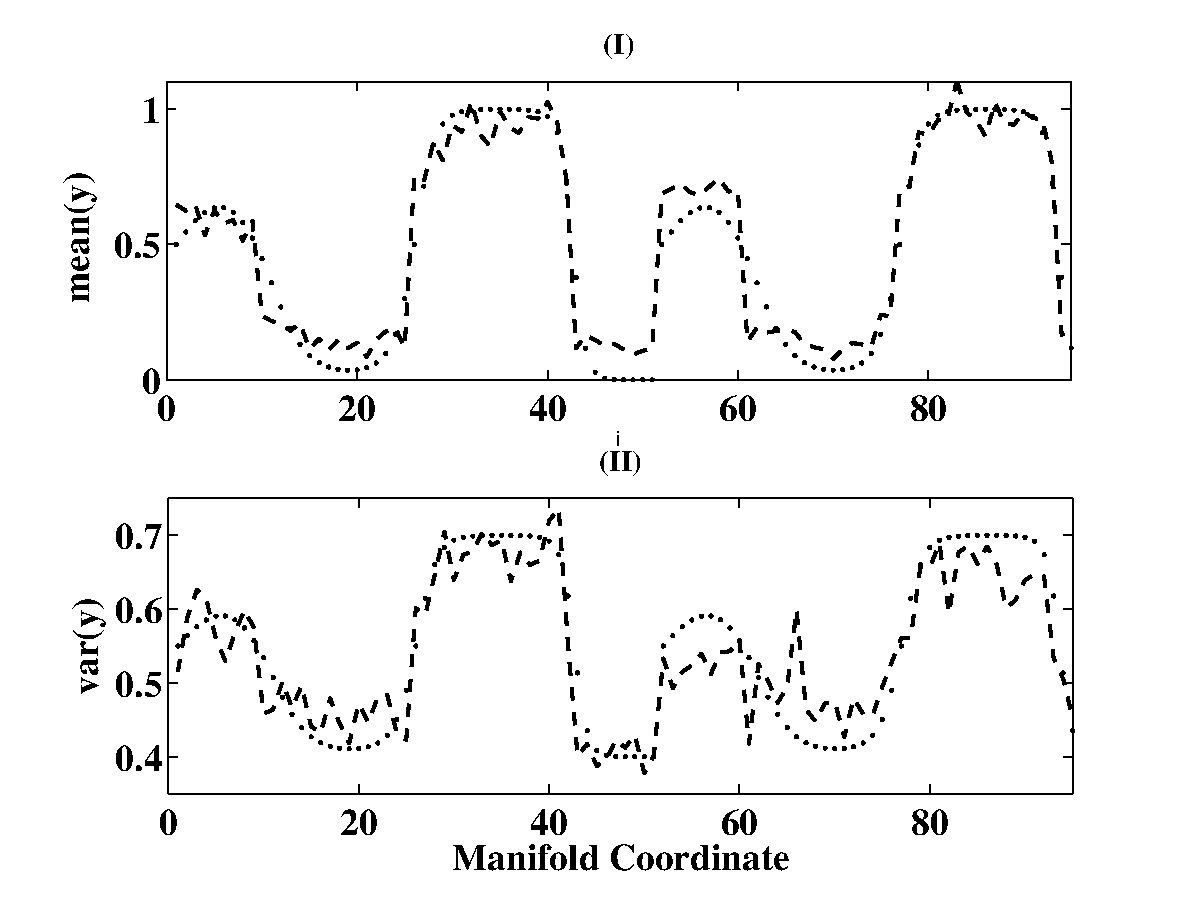
\includegraphics[width=70mm,height=30mm]{illustrativeExample.eps}
        \label{fig:second_sub}
    }
    \subfigure[]
    {
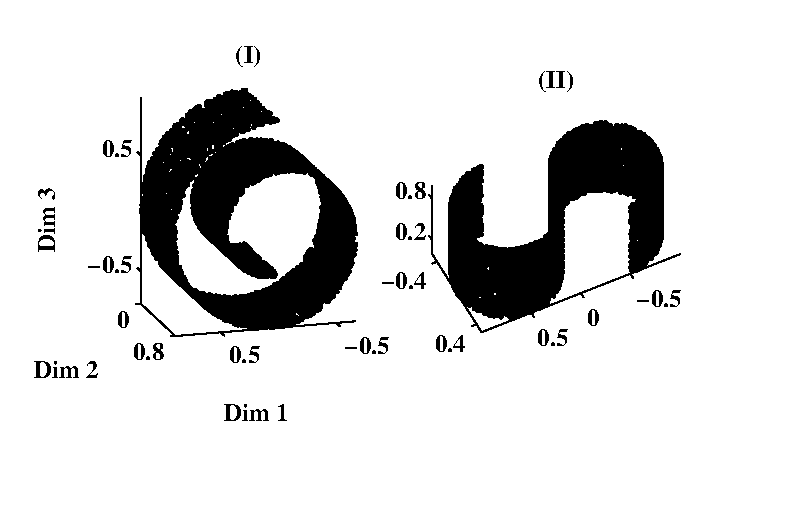
\includegraphics[width=70mm,height=30mm]{manifold.eps}
        \label{fig:third_sub}
    }
    \caption{(a) Plot of mean and variance (I-II) for observations $i=1, \ldots, 95$ (dot:true, dash:estimate); (b) Toy data examples: Swissroll (I) and S-Manifold (II) embedded in $\mathcal{R}^3$}
    \label{fig1}
\end{figure}
%
%\begin{figure}
%\centering
%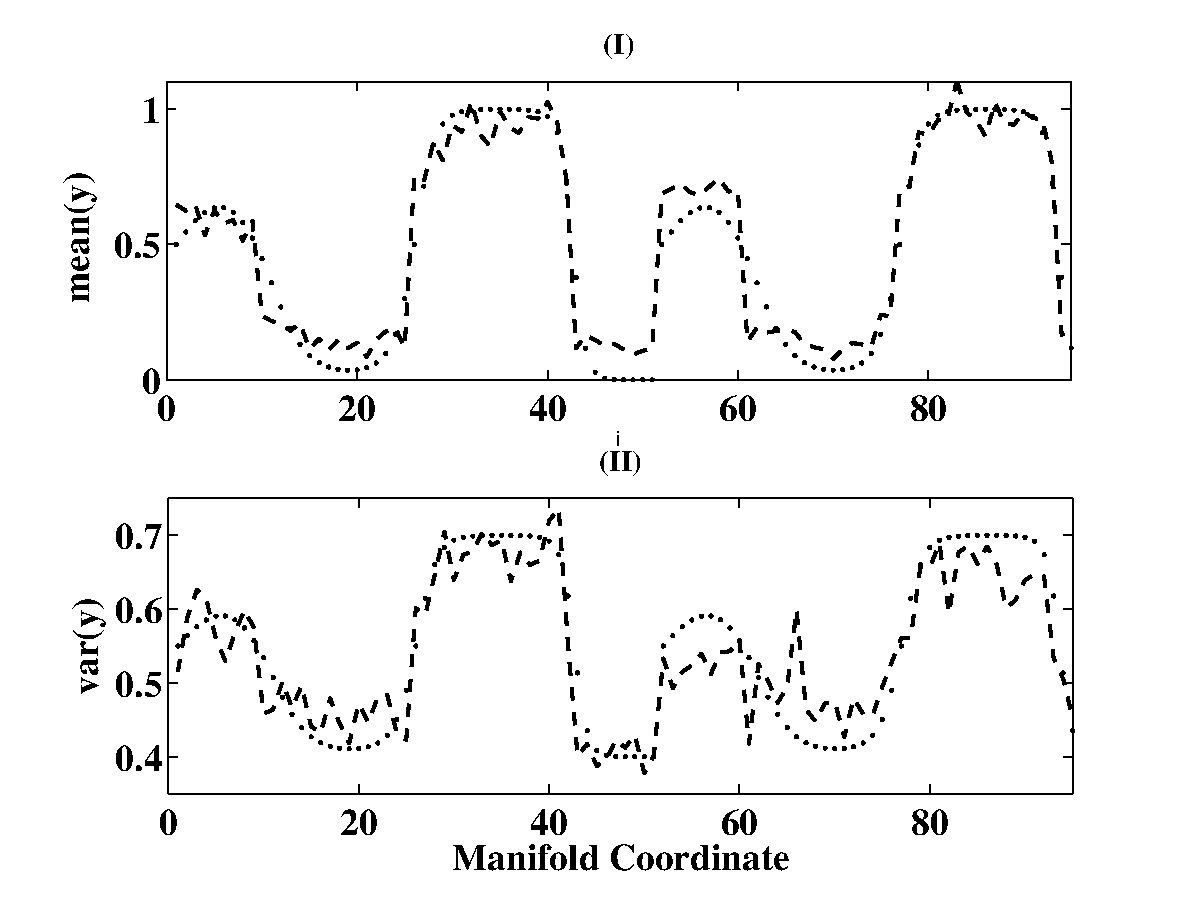
\includegraphics[width=80mm,height=30mm]{illustrativeExample.eps}
%\caption{ Plot of mean and variance (I-II) for observations $i=1, \ldots, 95$ (dot:true, dash:estimate)} \label{fig:wave}
%\end{figure}



In all other examples, predictors were assumed to belong to a lower dimensional space, either a lower dimensional plane or a non linear manifold. For each synthetic dataset, the proposed model was compared with CART and lasso in terms of mean squared error. In the first three simulation studies, the vector of predictors was assumed to lie close to a lower dimensional plane. In practice,  predictors were modeled through a factor model, i.e. $x_i=\Lambda \eta_i + \epsilon_i$ with $\epsilon_i \sim \mc{N}_n(0,\mb{I}_n)$, $\Lambda$ being a $(p \times r)$ matrix, $\eta_i \sim \mc{N}_r(0,\mb{I}_r)$ and $r<<p$. The response $y$ was assumed to be a function of the latent variable $\eta$ so that  the dependence between response and predictors was induced by the shared dependence on the latent factors.  In all examples, $\Lambda$ was assumed to be a sparse matrix with level of sparsity increasing with the number of columns and non zero elements of $\Lambda$ drawn from a standard normal density. In the last two simulation studies, predictors were assumed to lie close to the swissroll and the S-manifold (see figure \ref{fig1}(b)).
%
%\begin{figure}
%\centering
%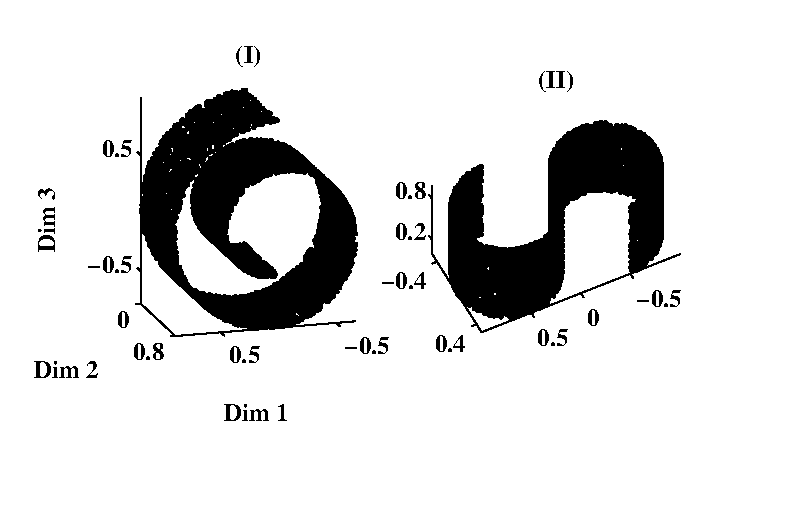
\includegraphics[width=70mm,height=40mm]{manifold.eps}
%\caption{Toy data examples: Swissroll (I) and S-Manifold (II) embedded in $\mathcal{R}^3$} \label{manifold}
%\end{figure}


In the first simulation study, $(r,p)$ were chosen to be $(5,1000)$ and response and predictors were jointly sampled from the above factor model.  In the second simulation study, $(r,p)$ were chosen to be $(5,10000)$ and the response was drawn from a two components mixture of normals with mixture weights depending on the first latent factor, i.e. $p=\exp\{\eta_1)/(1+\exp(\eta_1)\}$, and components with location parameters $(-2,2)$ and unitary standard deviation.  In the third simulation study, $(r,p)$ were chosen to be $(5,5000)$ and the response was drawn from a normal with mean and variance depending on the first latent factor as follows $y \sim \mc{N}\{\eta_1^2-\eta_1^3, \exp(1-\eta_1)\}$. In the last two simulation studies, predictors were drawn from the swissroll and the S-manifold, all two-dimensional manifolds but embedded in $\mathcal{R}^{50}$, while the response was sampled from a normal with mean equal to one of the coordinates of the manifold and standard deviation one.

Table \ref{table1} shows mean squared errors under the proposed approach, CART and lasso based on leave-one-out prediction. In particular, for each resolution level, the new observation was allocated to the set with closer center. As shown in table \ref{table1}, CART performs worse than lasso only when the response is a linear function of predictors. However, in all data scenarios, our model is able to perform as well as or better than the model associated to the lowest mean squared error. Moreover, as shown in figure \ref{Cpu}, our approach scales substantially better than competitors to massive number of features. Figure \ref{Cpu} shows the plot of CPU usage as a function of the number of features. This plot was obtained drawing $(y_i, x_i)$, for $i=1, \ldots, 100$, and $x_i \in \mathcal{R}^p$  from the first simulation scenario considering different values of $p$.
\begin{table}[t]
\caption{Mean and standard deviations of squared errors under multiscale stick-breaking (MSB), CART and Lasso for sample size 50 and 100}
\label{table1} \vskip 0.15in \begin{center} \begin{small} \begin{sc}
\begin{tabular}{llllllllllllllllll}
\hline
\abovespace\belowspace
 model&& msb&cart&lasso\\
\hline
\\
(1)&mse&     1.09 & 2.29 & 1.09\\
& & \begin{scriptsize} (1.68)\end{scriptsize} & \begin{scriptsize} (2.82)\end{scriptsize}& \begin{scriptsize} (1.66)\end{scriptsize}\\

(2)&mse&0.55& 0.55 &0.99\\ 
&& \begin{scriptsize} (0.86)\end{scriptsize} & \begin{scriptsize} (0.62)\end{scriptsize} & \begin{scriptsize} (0.79)\end{scriptsize}\\
(3)&mse&  0.78 &0.83 & 0.84\\
&&   \begin{scriptsize} (1.99)\end{scriptsize} & \begin{scriptsize} (2.16)\end{scriptsize} & \begin{scriptsize} (2.00)\end{scriptsize}\\
(4)&mse& 0.80&1.00&1.01 \\
&& \begin{scriptsize} (0.82)\end{scriptsize}& \begin{scriptsize} (1.36)\end{scriptsize}& \begin{scriptsize} (1.04)\end{scriptsize}\\
(5) &mse & 0.60&0.64 &1.01\\  
&& \begin{scriptsize} (0.76)\end{scriptsize}& \begin{scriptsize} (0.84)\end{scriptsize}& \begin{scriptsize} (1.16)\end{scriptsize}\\
\\
\hline
\end{tabular}
\end{sc}
\end{small}
\end{center}
\vskip -0.1in
\end{table}

Another important advantage of the proposed model is the possibility to obtain an estimate of the predictive density of the data. Figure \ref{plotDensity} shows the estimated density of two data points sampled from the second simulation scenario. Clearly, the density function varies based across different points and our estimate become closer to the true density as the number of observations in the training set increases.



\begin{table}[t]
\caption{Real Data: Mean and standard deviations of squared error under multiscale stick-breaking (MSB), CART, Lasso and random forest (RF)}\label{real} \vskip 0.15in \begin{center} \begin{small} \begin{sc}
\begin{tabular}{llllllllllllllllll}
\hline
\abovespace\belowspace
data  &model&mse&$t_{T}$ & $t_{M}$ & $t_{V}$\\
\hline
\\
(1)&msb &$0.56$ & $100$ & $1.1$& $0.02$\\
 & cart & $1.10$ & $87$ & $0.9$ &$0.01$\\
& lasso & $0.63$  & $200$ & $2.8$ & $0.17$\\
& rf & $0.57$ &  $7,817$ & $78.2$ & $0.59$\\
\\
(2)&msb &$0.76$ & $690$ & $20.98$& $2.31$\\
 & lasso & $1.02$  & $5,836$ & $96.18$ & $9.66$\\
\\
\hline

\end{tabular}
\end{sc}
\end{small}
\end{center}
\vskip -0.1in
\end{table}

\section{Real Application}

We assessed the predictive performance of the proposed method on two real datasets. The first dataset consists of a measurement of creativity observed for $108$ subjects. We would like to predict the value of creativity based on the number of connections between different cortical regions of the brain. Therefore, for each subject, a brain graph involving $70$ cortical regions was observed. The vector of covariates consists in the logarithm of the total number of connections between all pairs of cortical regions, i.e. $p=2,415$. The second dataset consists of a measure of head motion observed for $56$ subjects. As a measure of head motion we considered the mean framewise displacement (FD) computed as described in \cite{Power}. Our interest was predicting the head motion measurement based on $3$D brain images involving about $1$ million of pixels.  In order to reduce the dimensionality of this problem we reprocessed the data using a brain mask \francy{say something here} . After processing the data, we obtained a vector of about $300,000$  pixels that we considered as covariates in our model.

For the analysis all variables have been normalized by subtracting the mean and dividing by the variance. The same prior specification and Gibbs sampler as in \S 5 was  utilized. Table \ref{real} shows mean and variance squared error based on leave-one-out predictions. Variable $t_{T}$ is the amount of time necessary to obtain predictions for all subjects, while variables $t_M$ and $t_V$ are respectively the mean and the variance of amount of time necessary to obtain prediction for one subject.

 For the first data example, our model was compared to CART, lasso and random forest. As shown in table \ref{real}, our approach is able to perform better than random forest in terms of mean squared error and is associated to a much lower CPU time. It is important to note that this real data example does not involve a huge number of predictors so that computationally our model performs almost as well as lasso and CART. However, as we have shown in section 5, our model can scale substantially better than all other models to huge number of features. \\
 
 For the second data application, given the huge dimensionality of the predictor space and the poor scalability of CART and random forest, the comparison was made only with lasso. As shown in table \ref{real}, our approach is more efficient and accurate than lasso in predicting the response variable. Figure \ref{fig:real} shows the plot of CPU time used to predict each one of the $56$ subjects involved in the experiments. The time utilized to compute quantities calculated one time and used in all predictions was divided equally across subjects. Clearly, our approach is able to improve the computational time by up to five orders of magnitude.


\newpage
\nocite{langley00}



\begin{figure}
\centering
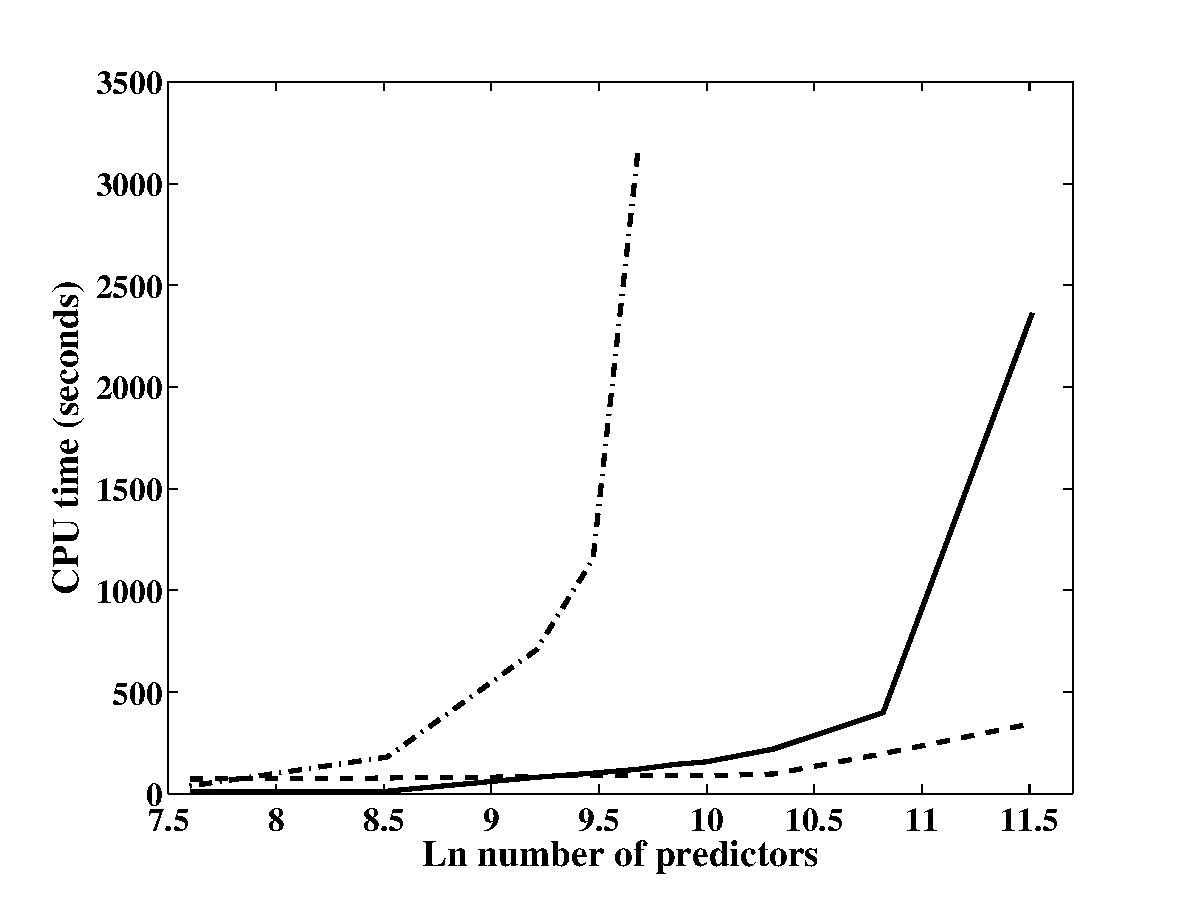
\includegraphics[width=80mm,height=35mm]{Cpu.eps}
\caption{Elapsed CPU time (in seconds) for leave-one-out prediction based on $100$ observations for MSB (solid), lasso (dash) and CART (dot-dash) for different number of predictors in log-scale} \label{Cpu}
\end{figure}

\begin{figure}
\centering
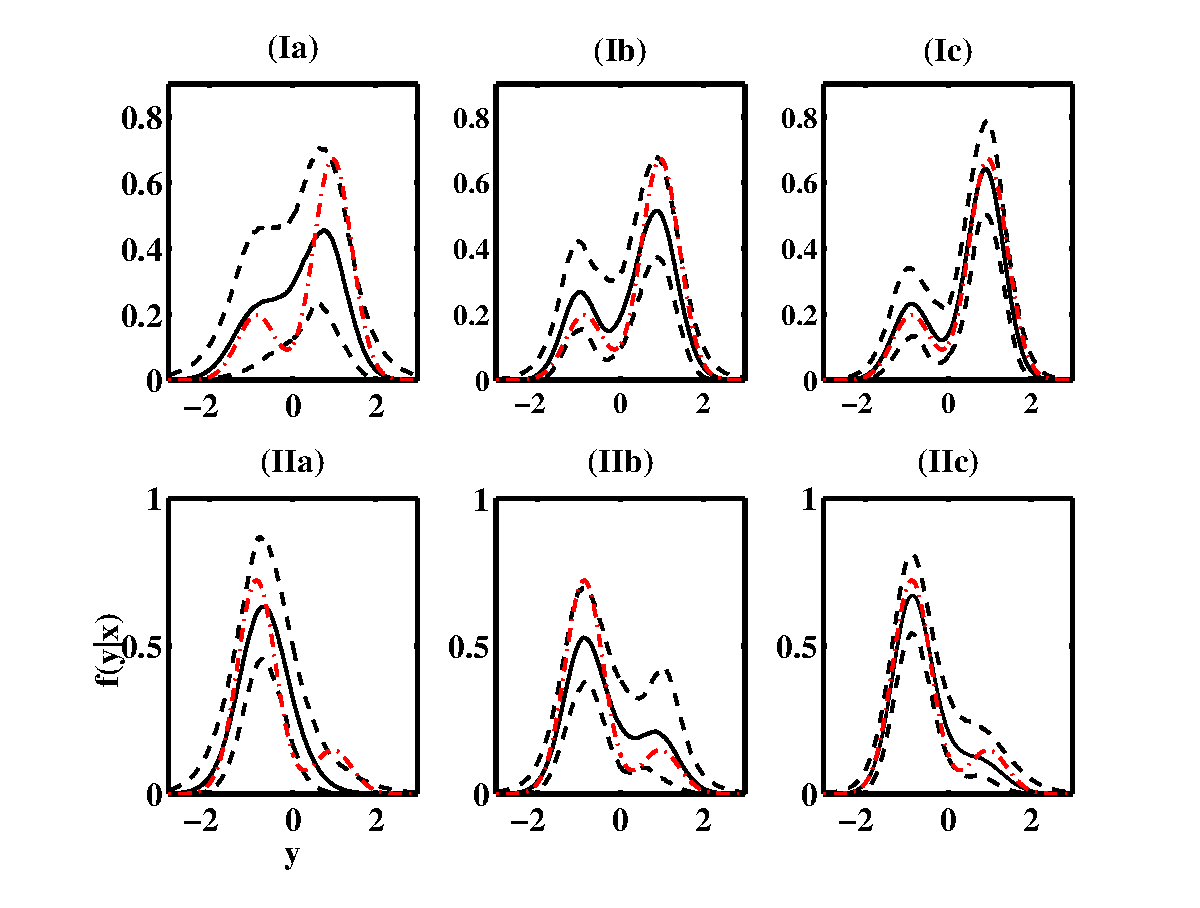
\includegraphics[width=85mm,height=60mm]{densityestimate.eps}
\caption{Plot of true density (dashed-dotted line) and estimated density ($50$th percentile: solid line, $2.5$th and $97.5$th percentiles: dashed lines) for two observations $(I, II)$ considering different training set size (a:50, b:100, c:150). } \label{plotDensity}
\end{figure}

\begin{figure}
\centering
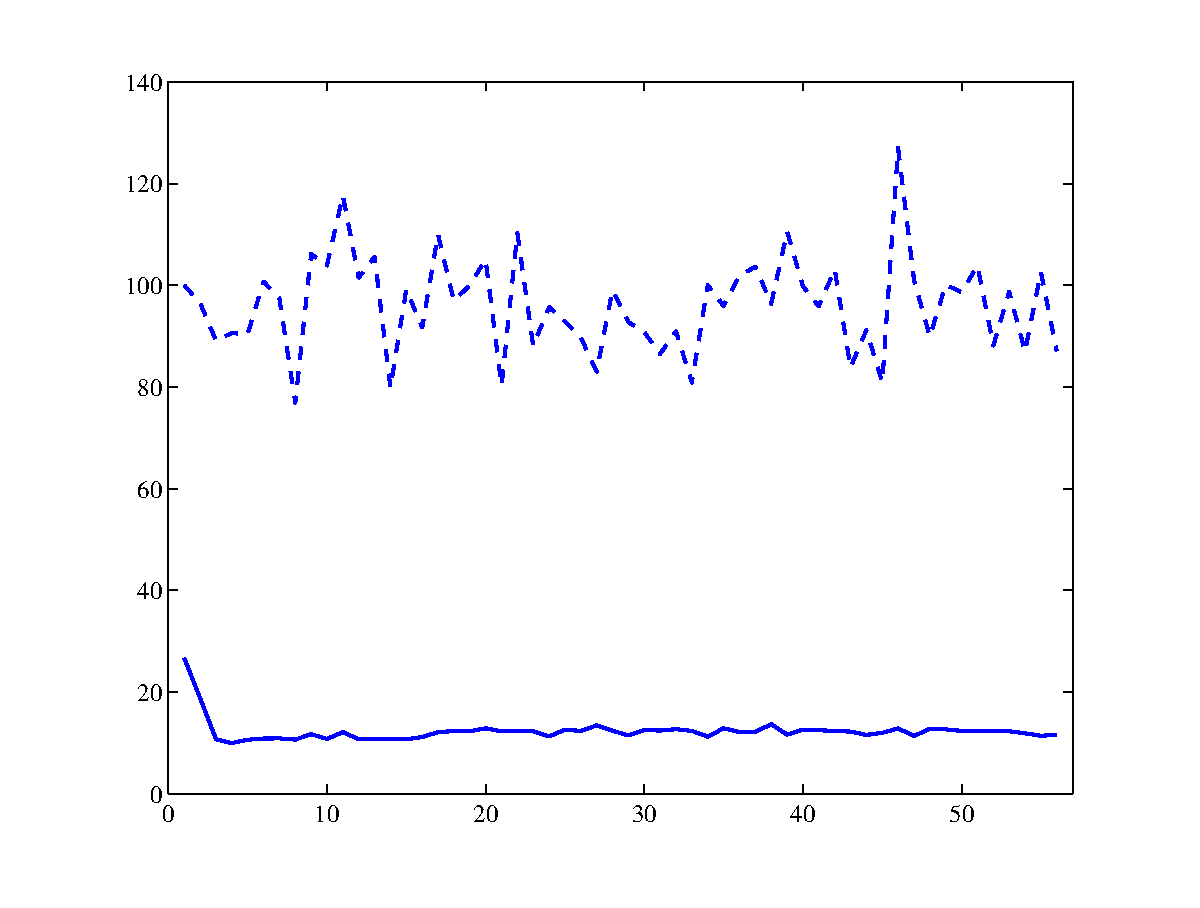
\includegraphics[width=80mm,height=30mm]{Time_real.eps}
\caption{Plot of CPU time used to predict each one of the $56$ subject involved in experiment (2) under MSB (solid) and lasso (dash)} \label{fig:real}
\end{figure}


\section*{Discussions}
We have proposed a new model which should lead to substantially improved predictive and computational performance in general applications involving a set of high dimensional predictors. As shown, the proposed two stage approach can scale substantially better than other existing algorithms to massive number of features. We have focused on Bayesian MCMC-based methods, but there are numerous interesting directions for ongoing research.

\section*{Acknowledgments}
This research was partially supported by grant 5R01-ES-017436-04 from the National Institute of Environmental Health Sciences (NIEHS) of the National Institutes of Health (NIH) and DARPA MSEE.


\bibliography{multiscale6}
\bibliographystyle{icml2013}
\end{document} 

